\section{Introduction}


\subsection{The IR camera}
Electromagnetic radiation of wavelengths between $700$ nanometer to
$1$ millimeter comprise what is usually referred to as
\textit{infrared light}. Much like the normal camera is able to detect
and display variations of visible light ($400$ nanometers to $700$
nanometers), infrared cameras produce pictures colored
according to the variations in infrared radiation (IR) of a
scene. Since infrared emission from an object is closely related to
its temperature, an IR camera essentially produces a heat map to the
eye, coloring parts of a scene relative to temperature. For instance
in Figure~\ref{fig:cat}, a cat is depicted based on the IR radiation
it emits. Many infrared
cameras are also able to accurately estimate the temperature of an
object in addition to depicting it.


\begin{figure}[h]
\begin{center}
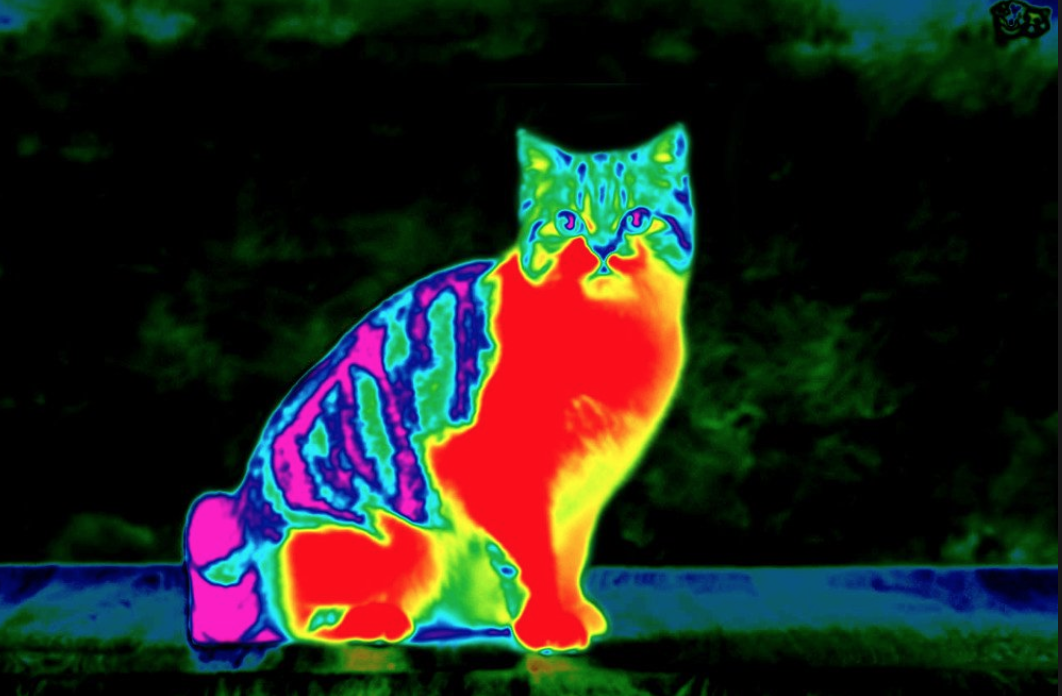
\includegraphics[height=5cm]{gfx/cat.png}
\caption{Infrared picture of a cat sitting on a table during
  night. The warmblooded cat is clearly distinguished from its cold
  surrounding, making the cat visible to the IR camera although not
  visible to the eye. Source:
  https://www.scienceabc.com/}~\label{fig:cat}
\end{center}
\end{figure}

Infrared cameras are used widely within industrial and military
applications, enabling or enhancing tasks such as dark vision, heat
leakage detection, moisture detection, chemical spill leakage
detection and firefighting. An overview about different devices
together with a catalog can be found in~\cite{flir_handbook}. There
exist mainly two types of techniques for infrared cameras: thermal
detectors and quantum detectors. We will here focus solely on thermal
detectors, and especially the \textit{uncooled bolometer}. A bolometer consists of a plate (pixel)
made of metal or semiconductor material, which for instance could be a mixture of
silicon nitride and vanadium oxide. This plate suspended in the air
via two supporting legs that is connected to a substrate. The
supporting legs are also connected to a voltage
source. The structure is depicted in Figure~\ref{fig:structure}. Incoming infrared radiation is focused via a lens to the
plate, causing it to be heated, which in turn alters its
resistance. This change in resistance can be measured through an
input voltage and the resulting current is a function of the strength
of the incoming infrared radiation and hence
the temperature of the emitting scene.

\begin{figure}[h]
\begin{center}
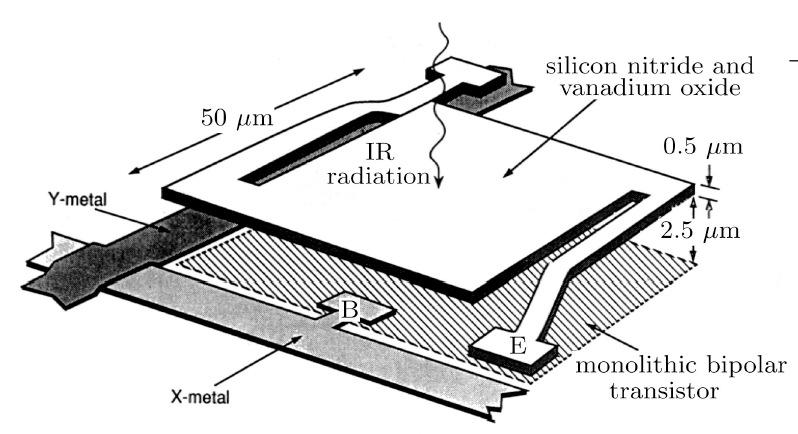
\includegraphics[height=5cm]{gfx/pixel1.png}
\caption{Physical structure of the bolometer~\cite{xiu2010research}.}~\label{fig:structure}
\end{center}
\end{figure}

\subsection{Project description}

The project aims to establish a mathematical relationship between the
temperature of an object and the resulting bolometer signal. Breifly,
the incoming radiation of an object, described by the Stefan-Boltzmann
law, heats up the bolometer, which can be described by the heat
equation. The applied voltage is used to measure the change in
resistance due to the temperature change. More precisely, the
output signal is a voltage from an integrator, that can be used to
retrieve the change in the resistance and thus via the heat equation
and the Stefan-Boltzmann law the temperature of the target. An explicit
description of the output signal is given in
Section~\ref{sec:model_disc}.


%By solving the ODE's numerically, we can get the output signal $v_s$ as a deterministic function of $T_o$. In reality however, the output signal $v_s$ is noisy. The project aims to incorporate noise into the model in a manner consistent with data and experience. A good model of the noisy signal might for example enable an efficient filtering that reduces noise.

In reality however, the output signal is noisy. The project aims to incorporate noise into the model in a manner consistent with data and experience. A good model of the noisy signal might for example enable an efficient filtering that reduces noise. The project's aim is to investigate how a noisy input signal effects the output signal.

More precisely in this project we:
\begin{itemize}
 \item simulate the read-out signal of the bolometer by solving the differential equations modeling the problem,
 \item reproduce numerical simulations that fits with empirical experiments,
 \item model and analyze the noise in the differential equations,
 \item reproduce numerical simulations (with noise) that fits with empirical experiments.
\end{itemize}

%%% Local Variables:
%%% mode: latex
%%% TeX-master: "main"
%%% TeX-PDF-mode: 1
%%% TeX-PDF-via-dvips-ps2pdf: 1
%%% End:
